\documentclass[11pt]{article}
%Gummi|063|=)

\usepackage{ntheorem}
\usepackage{amssymb}
\usepackage[T1]{fontenc}
\usepackage[utf8]{inputenc}
\usepackage{amsmath}
\usepackage{graphicx}

\newcommand{\RN}[1]{\uppercase\expandafter{\romannumeral #1\relax}}
\renewcommand\thesubsection{\thesection\alph{subsection})}



\title{\textbf{Econometrics Take Home Exam 2}}
\author{Johannes Degn 01/848553}
\date{18.01.2012}

\theoremstyle{break}

\begin{document}
\maketitle


\section{Problem}
Random Seed for the whole problem: "rndseed 1;"

\subsection{}
Heteroskedasticity means that the dependent variable of each observation has a potentially different variance depending on the independent variable. I.e. the conditional variance $V(Y|X)$ differs. If we use the model $Y_i = \beta X_i + \varepsilon_i$ the variance of $\varepsilon_i$ carries an index $i$ to denote that it differs among observations. One simple example where this might occur is if $X$ denotes gender (where $Y$ can denote e.g. income) and we observe that the variance among the income of the male observations is different to the variance of the female observations.

This is an issue because the estimates for the variance of the parameters and thus the estimates for the standard errors might be too small compared to robust estimates. As a result hypothesis tests might yield wrong results.


\subsection{}
Let $A(X_i) = X_i\exp(-X_i)$ be the matrix of instruments and let $\rho(Z_i, \beta) = \varepsilon_i = (Y_i - X\beta)$. $\rho(Z_i, \beta)$ is a well defined conditional moment function for $\tilde{\beta}$ since $E(\rho(Z_i, \beta)| X_i) = E(\varepsilon_i | X_i) = 0$. Then $\psi(Z_i, \beta) = A(X_i)'\rho(z_i, \beta) = \exp(-X_i)X_i(Y_i-\beta X_i)$
\\
$\psi(Z_i, \beta) = \exp(-X_i)X_i(Y_i - \beta X_i)$ is a moment function that corresponds to $\tilde{\beta}$. $\psi(Z_i, \beta)$ is a well defined moment function because $E(\psi(Z_i, \beta)) = E(\exp(-X_i)X_i\varepsilon_i) = \underset{x}{E}(E(\exp(-X_i)X_i\varepsilon_i|X_i)) = \underset{x}{E}(\exp(-X_i)X_iE(\varepsilon_i|X_i)) = 0$. \\

Since we have $q=1$ moment function and $k=1$ parameter, we can simply replace the population moments with the sample moments in order to get a method of moments estimator: \\
$$E(\psi(Z_i, \beta)) = 0$$
$$E(\exp(-X_i)X_i(Y_i -X_i\beta)) = 0$$
$$\frac{1}{n}\displaystyle \sum_{i=1}^n(\exp(-X_i)X_i(Y_i -X_i\tilde{\beta})) = 0$$
$$\displaystyle \sum_{i=1}^n(\exp(-X_i)X_iY_i) = \displaystyle \sum_{i=1}^n(\exp(-X_i)X_i^2\tilde{\beta})$$
$$\tilde{\beta} = \frac{\sum_{i=1}^n(\exp(-X_i)X_iY_i)}{\sum_{i=1}^n(\exp(-X_i)X_i^2
)}$$


\subsection{}
From proposition 5.2.1 from the lecture notes it follows that $\sqrt{n}(\tilde{\beta}_n-\beta) \;{\buildrel d \over \rightarrow}\; N(0, E(\frac{\partial \psi(Z_i, \beta_0)}{\partial \beta'})^{-1})V_0 E(\frac{\partial \psi(Z_i, \beta_0)}{\partial \beta})^{-1})$
and $\tilde{\beta} \;{\buildrel d \over \rightarrow}\; N(\beta_0, E(\frac{\partial \psi(Z_i, \beta_0)}{\partial \beta'})^{-1}\frac{V_0}{n} E(\frac{\partial \psi(Z_i, \beta_0)}{\partial \beta})^{-1})$. \\

In our case we have $V_0 = V(\psi(Z_i, \beta_0)) = E(\psi(Z_i, \beta)^2) = E(\exp(-2X_i)\varepsilon_i^2X_i^2) = E(\underset{x}{E}(\exp(-2X_i)\varepsilon_i^2X_i^2|X_i)) = E(\exp(-2X_i)X_i^2\underset{x}{E}(\varepsilon_i^2|X_i)) = E(\exp(-X_i)X_i^2)$ and $\frac{\partial \psi(Z_i, \beta_0)}{\partial \beta'} = -\exp(-X_i)X_i^2$. \\
Thus: \\
$V(\tilde{\beta}) = E(-\exp(-X_i)X_i^2)^{-1}\frac{E(\exp(-X_i)X_i^2)}{n}E(-\exp(-X_i)X_i^2)^{-1} = \frac{E(\exp(-X_i)X_i^2)^{-1}}{n}$. Replacing the population moment with the sample moment yields the given variance estimator: \\
$\hat{V}(\tilde{\beta}) = \frac{1}{n}\frac{1}{\frac{1}{n} \sum_{i=1}^n\exp(-X_i)X_i^2}$.

\subsection{}
I expect both estimators to be consistent which can be seen either by taking the plim or since the asymptotic distribution of $\hat{\beta}$ and $\tilde{\beta}$ have expectation of $0$. The precision of an estimator is inverse to the variance. $\hat{\beta}$ is the White variance estimator for OLS which we know to be inefficient for for a model with heteroscedasticity. $\tilde{\beta}$ is an MM estimator for which we have: $E(\psi(Z_i, \beta)) = 0$. Since we have $\varepsilon_i = Y_i - \beta X_i \;{\buildrel d \over \rightarrow}\; N(0, \exp(X_i))$. The log likelihood function for $\varepsilon$ is $\ln L(Z_i, \beta) = -\frac{n}{2}\ln(2\pi\sigma^2) - \frac{(Y_i - \beta X_i)^2}{2\exp(X_i)}$ and the score function is $S(\beta) = \exp(-X_i)X_i(Y_i-\beta X_i)$. This is equivalent to the moment function we used earlier. We can thus see the moment estimator derrived earlier as a maximum likelihood estimator which we know to be efficient as it reaches the Cramer-Rao lower bound if the information equality holds.

\subsection{}
See Gauss code

\subsection{}
For the simulation: see Gauss code. \\
\begin{figure}[H]
\centering
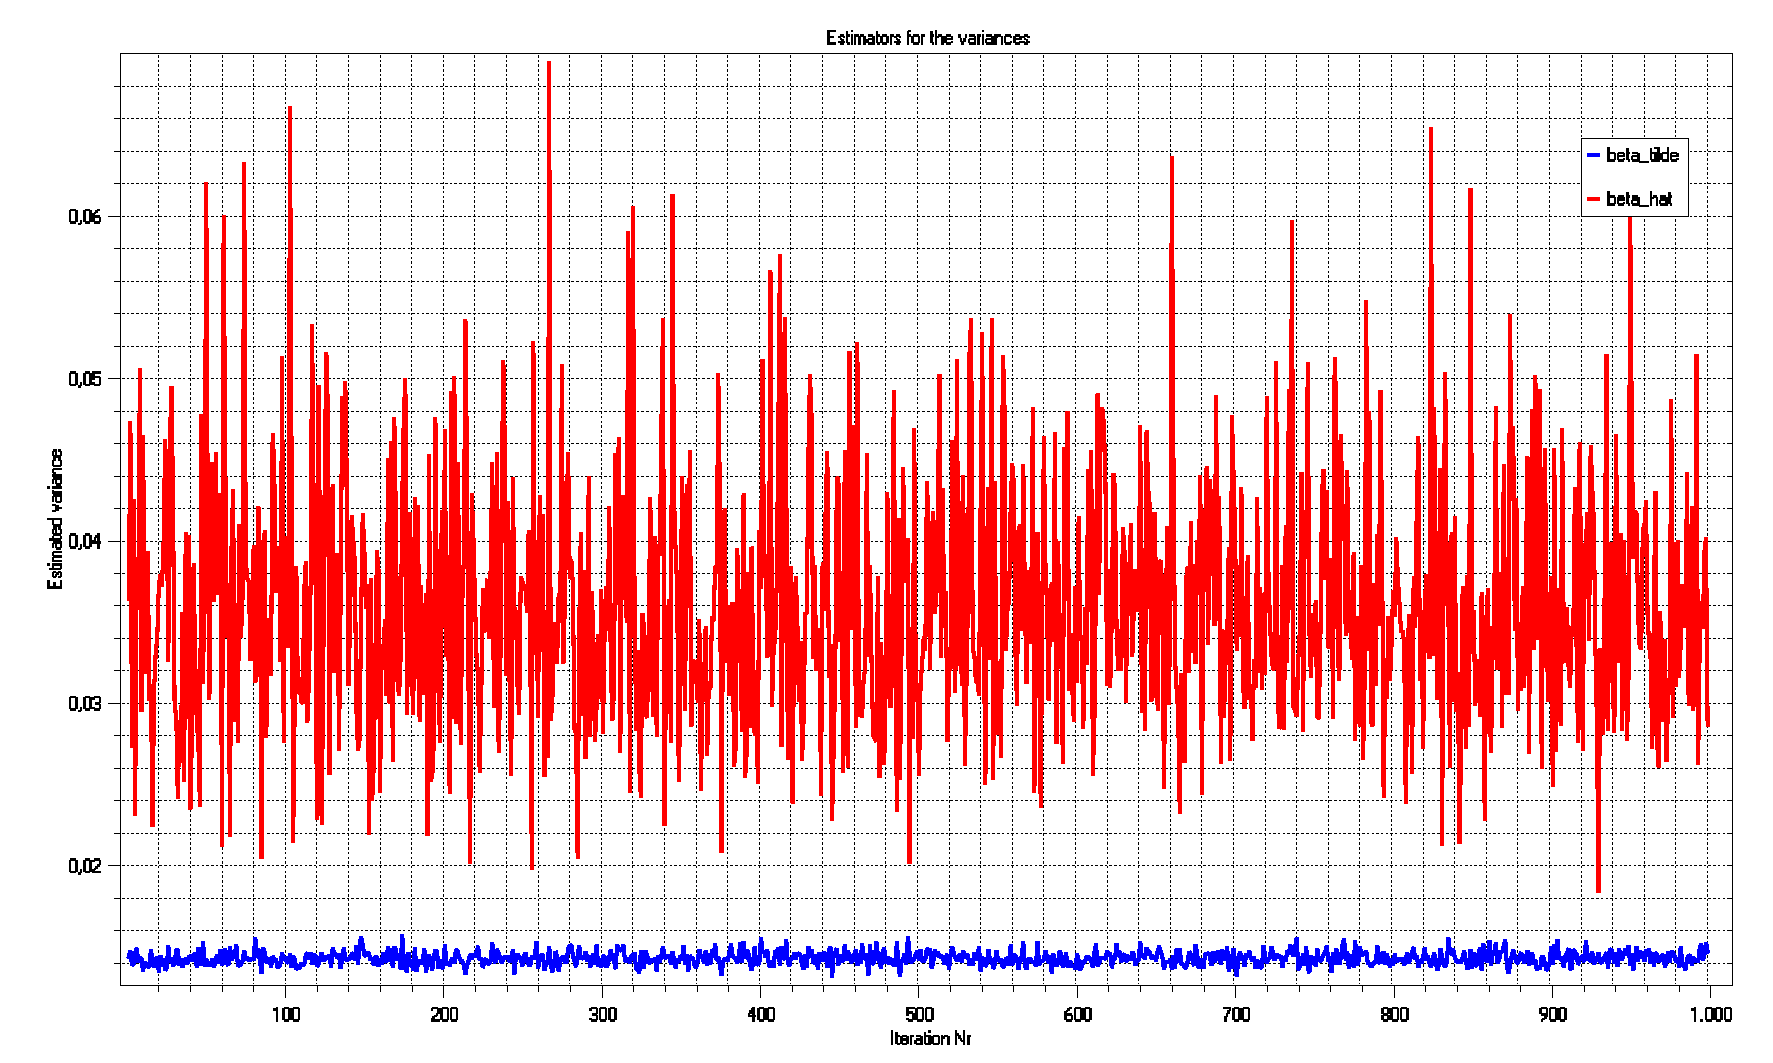
\includegraphics[height=100mm]{variance_estimators.pdf}
\caption{estimated variances}
\end{figure}
From the results we see that that both $\hat{\beta}$ and $\tilde{\beta}$ are consistent and approach 1 for large $R$ and $n$. As proposed, the values of $\hat{V}(\tilde{\beta})$ are smaller than the average $\hat{V}(\hat{\beta}))$. From the plot we can see that this holds generally and not only on average. \\
The lower variance estimates for $\hat{V}(\tilde{\beta})$ result in higher t-statistics which lead to higher rejection rates in the test with $H_0:\beta=0.8$


\end{document}